\chapter*{Pista de carreras}
\section*{Pista de carreras}
a)Mostrar que es posible construir una pista de un cuarto de milla alrededor del
campo de football. (Se sugiere calcular la longitud de la pista más corta que podría
construirse alrededor del campo).

\vspace{0.1cm}

La pista se compone de dos secciones, la sección uno que serían las dos partes rectas y los dos semicírculos. La longitud mínima de las rectas de la pista deben medir lo mismo que el largo de la cancha que es $360ft$, por otra parte, ambos semicírculos, el diámetro mínimo lo consideramos como la anchura de la cancha que es de $160ft$
Sabemos que la circunferencia de un círculo se obtiene con la fórmula $C=\pi d$ donde $d$ es el diámetro.
Entonces, para poder construir la pista con la minima distancia es necesario sumar las dos longitudes a lo largo de la pista más la circunferencia de los dos semicírculos.
$$\Rightarrow L=\pi \cdot d + 2\cdot 360$$
Podemos poner la formula completa ya que los dos semicírculos son iguales y forman un circulo completo de diámetro $160ft$.
Sustituyendo: 
\begin{gather*}
    L=\pi\cdot160ft+\cdot360ft\\
    L\simeq 1222.6548ft\\
\end{gather*}
Podemos notar que el valor dado para construirla pista con la longitud minima constituida por dos semicírculos y dos lados rectos es menor al requerido $1222.6548ft<1320ft$.
\vspace{0.2cm}

b) Sea L la longitud, en pies, de una de las partes rectas de la pista y sea x la distancia, en pies, entre la línea lateral del campo y una de las partes rectas de la pista. Muestre que L como función de x viene dada por:
$$L(x) = 660 - 80 \pi - \pi x$$

y grafique esta regla de correspondencia para $0 \leq x \leq 20$.
\vspace{0.2cm}

Para expresar L en función de x $L(x)$ aumentamos en x el diámetro de los semicírculos de la función de tal manera que: diámetro $$=160 + x$$
Ahora calculamos la circunferencia  $c=\pi*diametro\therefore c=\pi*(160+x)$

Sea $L$ la longitud de los lados rectos para las cuales queremos expresar la variabilidad de su comportamiento en función de $x$.
Entonces queremos saber en que x el valor será de la pista será $1320fts$ en la suma de las longitudes.
\begin{gather*}
    (160ft+x)\pi + 2L = 1320ft\\
    \pi\cdot160ft+\pi\cdot x + 2L = 1320ft\\
    2L = 1320ft - 160\pi ft -\pi x\\
    L=\frac{1320ft - 160\pi ft -\pi x}{2}\\
    L=660-80\pi - \pi x
\end{gather*}

$$\therefore L(x)=660 - 80\pi-\pi x$$

\begin{center}
        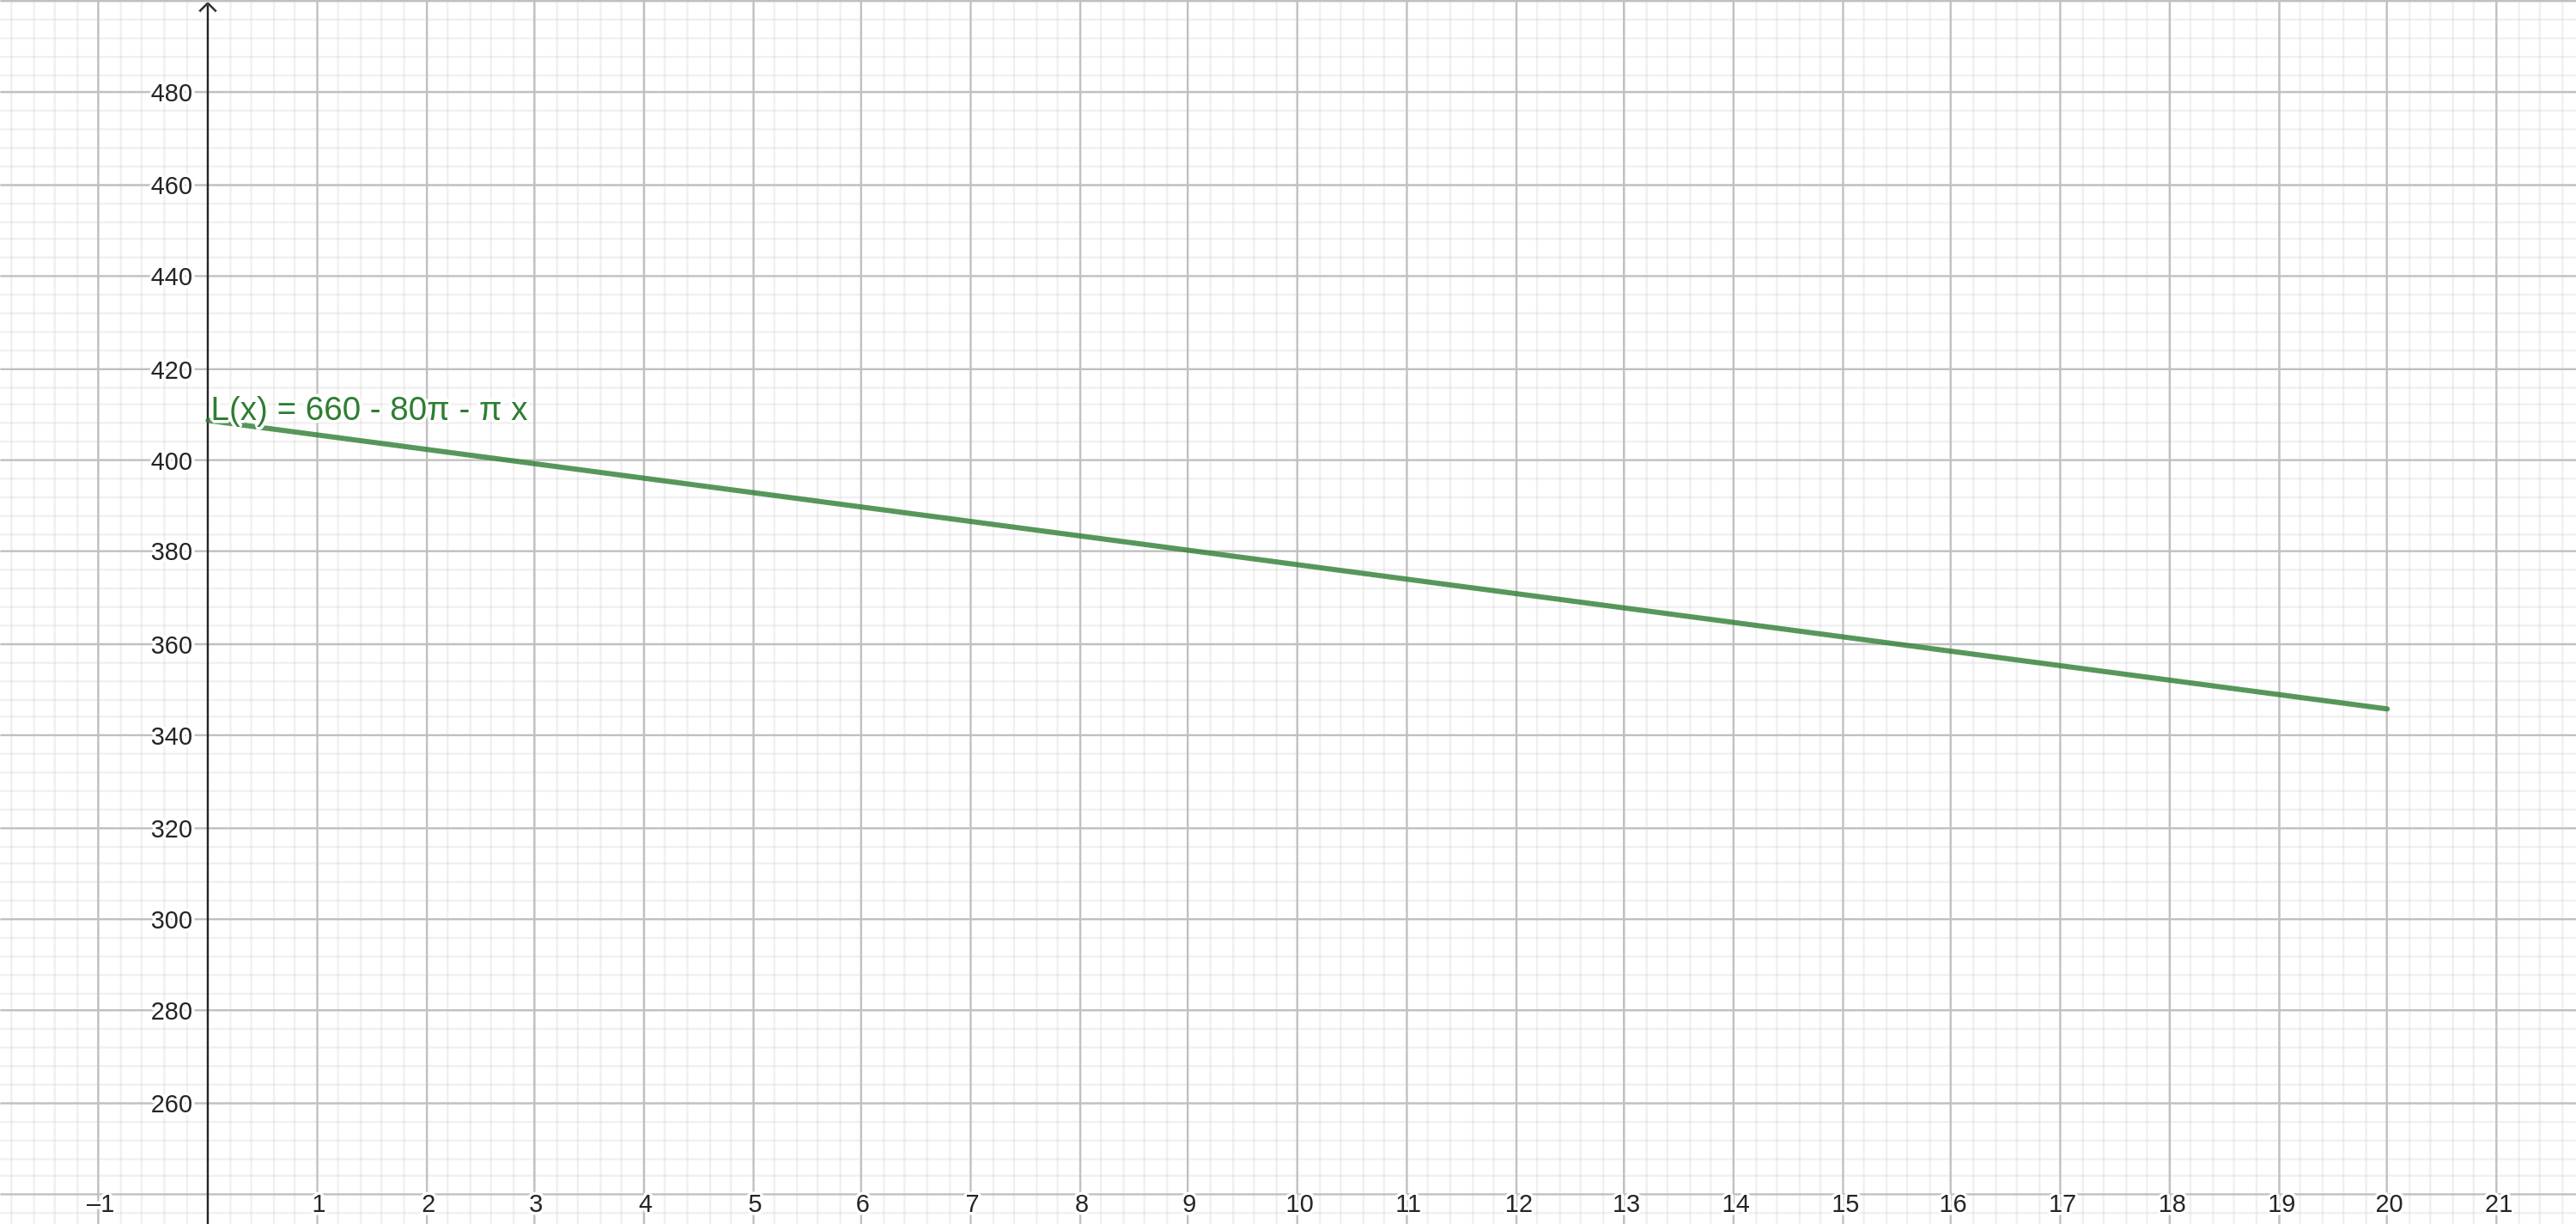
\includegraphics[height = 0.3\textheight]{recursos/geogebra-export.png}\par
\end{center}


Con base en esta
gráfica:

1) Estime la mínima longitud de la parte recta de la pista y, luego, muestre que el valor de x para el que ésta ocurre es aproximadamente 15.49 ft.

Tomando en cuenta que la longitud mínima que puede tomar la pista es de 360 debido a que es la misma longitud que mide el campo de football, queremos saber el valor de separación entre el campo y la pista para que la longitud total de la pista sea $\frac{1}{4}$ de milla = $1320ft$

\begin{gather*}
    360=660-80\pi-\pi x\\
    360-660+80\pi=-\pi x\\
    \frac{360-660+80\pi}{-\pi}=x\\
    \therefore x\simeq 15.49ft
\end{gather*}

$15.49ft$ debe ser la medida aproximada de la distancia entre la pista y el campo para que la pista tenga una Longitud total de $1320ft$.
\vspace*{0.2cm}


2) Estime la máxima longitud de la parte recta de la pista y luego, muestre que el valor de L para el que ésta ocurre es aproximadamente 408.67 ft.

El máximo valor de de la longitud de la parte recta debe ser cuando no hay separación entre el campo de fútbol y la pista, por tanto, debemos sustituir para $ L(0)$.
\begin{gather*}
    L(0)=660 - 20\pi-\pi(0)\\
    L(0)\simeq 408.67ft
\end{gather*}

$\therefore$ La longitud máxima de la parte recta de la pista debe medir $408.67ft$ para que la longitud total de la pista sea de $\frac{1}{4}$ de milla = $1320 fts$